\chapter{Background}

In this chapter, concepts, and terminology relevant to the thesis is explained, mainly, technological foundations such as \acrfull{ais}, conceptual foundations such as \acrshort{ais}-based trajectories and trajectory similarity measurements, and techniques applied to predicting future destination ports of traveling vessels, namely, \acrfull{ml}.

\section{Concepts}

This section describes the broader concepts that are important to the thesis's solution and later discussions. The section's purpose is to give the reader a base understanding of conceptual foundations and challenges the thesis later refers to.

\subsection{Vessel voyage definition}
\label{sec:vessel_voyage_definition}

In order to effectively predict a vessel's future destination, or analyze \gls{voyage} patterns in general, a vessel \gls{voyage} must first be defined. This definition is in the context of constructing voyages from \acrshort{ais} data and is a crucial concept to define since it affects the outcome of any prediction method that considers historical voyages and ensures comparability with existing work within this area of study. The main factor to define is when a vessel arrives at a port, or more specifically, the conditions that must hold in order to consider a vessel as having arrived at a specific port.

There might be several different reasons for a vessel to visit a port, not all of which means that the port was the vessel's final stop in a voyage. For instance, larger vessels traveling long distances, often have to bunker (refuel) at bunker ports between the port they loaded cargo at and the port they eventually will unload the cargo at. In some cases, vessels anchor outside of such bunker ports awaiting to be refueled by bunker vessels, while in other cases they can reduce their speed and be refueled without ever stopping completely. Another common reason for vessels to physically stop moving is congestion in ports. Very often vessels of any size have to wait their turn before loading or unloading at busy ports. It is also common that vessels have to wait to pass through narrow canals. In these cases, they might anchor closer to a different port than the final arrival port while they wait for access. However, under such circumstances, vessels may not consider themselves ``arrived'' as they intend to discharge their cargo at a different port. In either case, whether vessels refueling at bunker ports, or stopping for other reasons, should be considered arrivals or not ultimately depends on the desired outcome of future predictions and context.

For the purpose of this thesis, an arrival is defined only when the vessel herself claims to be moored by reflecting this as a navigational status in the \acrfull{ais} data. As vessels usually do not use the moored signal when bunkering, or for short stops along a voyage, this entails that the proposed solution will be more prone to predicting the final destination of a vessel even though it might stop for other reasons along the voyage. This voyage definition is thought to be more beneficial for people working in the shipping industry who are interested in knowing what vessels are available in different regions for chartering. However, a disadvantage is that fewer voyages can be constructed from the available data as longer voyages could have been divided into multiple smaller voyages if considering bunkering, for instance, as port arrivals.

A literature study, later described in \cref{sec:lit_review}, shows that there are few studies that consider voyage prediction, however, the most common alternative method of defining trajectories of vessels is to use some form of clustering. The most promising of these studies defined port arrivals by detecting clusters of vessel positions transmitted close to ports. In contrast to using navigational statuses, this method defines voyages as trajectories between stopping ports, thus voyages stopping mid-voyage at smaller ports were considered separate voyages. The main advantage of this characterization is that the constructed voyages are more easily comparable as they do not include any additional port visits along its voyage trajectory. When compared to the aforementioned definition based on navigational statuses, there could be more voyages constructed using the cluster-based approach as it has a lower threshold for considering a port visit an arrival. Therefore, in the context of a prediction model, there would be more voyage samples available for learning when using the cluster-based definition.

\begin{figure}[htbp]
    \centering
    \includegraphics[width=0.9\textwidth]{figures/mo_voyage}
    \caption{Example voyage, created using \acrshort{mo}'s route planner tool, for a traveling vessel (Pacific Harvest), traveling from Brazil to China while stopping at Singapore to refuel.}
    \label{fig:example_voyage}
\end{figure}

As an example, consider a voyage starting in Brazil and ending in Shanghai, China. Depending on the speed and fuel consumption of the traveling vessel, this voyage is around 12 000 nautical miles long and would take between 30 and 40 days. Thus, it is probable that a traveling vessel would stop to refuel at a bunkering port such as the one in Singapore. In this example (shown in \cref{fig:example_voyage}), one could either consider one complete voyage from Brazil to China, or one could consider two voyages; one going from Brazil to Singapore, and another going from Singapore to China. Assuming the vessel uses the navigational status ``moored'' in Brazil and China, but not in Singapore, the approach used in this thesis would consider one complete voyage from Brazil to Singapore, since it reflects the intended voyage while a clustering-based method, in contrast, would consider the two shorter voyages.

In this example, it is commercially more valuable for a prediction method to predict the vessel's destination to be in China rather than Singapore, since the fact that the vessel might stop to bunker at Singapore is somewhat obvious based on common sea lanes and voyages. This is the main reason for primarily focusing on the voyage definition using vessels' navigational statuses in this thesis.

\subsection{Trajectory similarity}
\label{sec:trajectory_similarity}

As will be further elaborated on in \cref{chap:related_work}, the current literature related to vessel destination predictions almost exclusively relies on some form of trajectory similarity. Vessels' current trajectory seems to provide good insight into their intended destination since vessels are unlikely to follow unique trajectories during a voyage. Vessels are more likely to either follow established shipping lanes or the most optimal and fuel-efficient route. Trajectory similarity measurements can be used to find the most similar historical trajectory to the current traveling trajectory to predict where the vessel will travel to. Therefore, trajectory similarity is also included in this thesis' proposed approach to vessel destination prediction as a method of considering spatial information as well as vessel details.

There are three main categories of trajectory similarity measurements: spatial, temporal, and tempo-spatial. Regarding vessel trajectories derived from \acrshort{ais}, they are not likely to share similar time intervals values as vessels travel at different speeds and at different times. Therefore, for the purpose of this thesis, only spatial trajectory similarity measures are considered. This assumption is further corroborated by \cite{Zhang2020AISApproach} that arrived at a similar conclusion in their work developing a \acrshort{ml} -based approach to trajectory similarity measurements.

There are a number of spatial trajectory comparison methods that have been widely used for different purposes. The most relevant are the Hausdorff distance \parencite{magdy2015}, Fréchet distance \parencite{magdy2015}, and \acrfull{sspd} \parencite{besse2015review}. Out of these, the \acrshort{sspd} method is the most appropriate as it handles trajectories of different shapes and lengths well which is beneficial when comparing a trajectory from an ongoing vessel voyage to a set of complete historical ones. \cref{fig:sspd} shows an example from \cite{besse2015review} where two trajectories are compared and their symmetric distances are calculated.

\begin{figure}[htbp]  % order of priority: h here, t top, b bottom, p page
    \centering
    \includegraphics[width=0.5\textwidth]{figures/sspd}
    \caption{Segment Path Distance (SPD) in the SSPD process of comparing two different trajectories \parencite{besse2015review}}
    \label{fig:sspd}
\end{figure}

Moreover, the \acrshort{sspd} method is available as a convenient Python library that also supports different algorithmic similarity measurement methods. For these methods, a distance function can be specified and used to calculate the distance between points in the algorithm. This is important as the trajectories are specified as geographical coordinates, and as these are spherical in nature, the most appropriate distance function is the Haversine \parencite{haversine} formula in contrast to the Euclidean formula commonly used for planar distances.

The methods mentioned thus far are all algorithmic approaches to measuring similarities between trajectories. However, there are also \acrshort{ml}-based methods as well such as the approach proposed by \cite{Zhang2020AISApproach} who also compare their results to the aforementioned methods.

They used a \acrfull{rf} model to measure trajectory similarity to find the most similar historical trajectory to any given traveling trajectory departing the same port. The most similar historical trajectory's destination is predicted to be the traveling vessel's destination. The study achieved a higher general accuracy level when compared similar approaches using algorithmic methods such as \acrshort{sspd}.

Moreover, some unsupervised clustering methods have also been applied to similar problems such as the \acrfull{dbscan} algorithm \parencite{dbscan} which is capable of sequentially finding patterns in points and trajectories. This approach is more frequently used in trajectory predictions on a small geographical extent such as for collision detection and anomaly detection.

\subsection{Machine learning (ML)}
\label{sec:machine_learning}

\begin{figure}[htbp]  % order of priority: h here, t top, b bottom, p page
    \centering
    \includegraphics[width=0.75\textwidth]{figures/ml-terms}
    \caption{Machine Learning (ML) hierarchical terminology}
    \label{fig:ml_terms}
\end{figure}

\acrfull{ml} is an umbrella term describing computer algorithms that automatically adapt and improve based on experience. Machine learning models are built based on a training dataset from which it derives patterns between underlying features. A trained model can be used to make predictions of a target value which can either be numerical or categorical.

There is a vast number of different \acrshort{ml} algorithms applied to different problem areas. \acrshort{ml} is mainly divided into three broad categories: supervised learning, unsupervised learning, and reinforcement learning. In supervised learning, in the training process, both input and the desired output are provided to the model. The model finds patterns and correlations between input and output data during the training process, and when the model is trained or fitted, it is capable of guessing output given only input.

In unsupervised learning, no output labels are provided to the model leaving the model to find patterns in the input set on its own. Clustering is an example of unsupervised learning as the model finds and labels patterns in input data without any external guidance. Reinforcement learning is a dynamic approach to \acrshort{ml} where the model continuously learns while trying to achieve a goal. In this method, the model navigates a problem space, and the program rewards or punishes the model that tries to optimize for rewards. In regards to topics covered by this thesis, \acrshort{ml}-based trajectory comparisons involve unsupervised learning, while predicting destination ports is supervised as the historical destinations are known.

\begin{figure}[htbp]  % order of priority: h here, t top, b bottom, p page
    \centering
    \includegraphics[width=0.75\textwidth]{figures/class_regg}
    \caption{Example showing the difference between classification and regression tasks}
    \label{fig:classification_regression}
\end{figure}

Moreover, supervised learning can further be divided into regression and classification problems. The main difference between the two is that classification aims at predicting a label, or a class, while regression predicts a quantity that is not necessarily present in the training data. For instance, a regression model can be used to predict the price of an item for sale, while classification can be used to label emails as "spam" or "not spam". \cref{fig:classification_regression} shows the difference between classification and regression. The example of classifying emails as ``spam'' or ``not spam'' would be considered a binary classification problem as there are only two possible labels, however, classification can also involve predicting more than two outcomes which are commonly referred to as multi-class classification. In the context of this thesis, predicting a vessel's destination port can be formulated as a multi-class classification problem as every possible destination port are different possible labels for a given voyage in progress. \cref{fig:ml_terms} shows how \acrshort{ml} is hierarchically divided into more specific terms relevant for the scope of this thesis.


\section{Technologies and protocols}

\subsection{Database system}

All the data that is used throughout this thesis for analysis is collected and stored in a \textit{PostgreSQL} database. \textit{PostgreSQL}, or \textit{Postgres}, is an open-source object-relational database management system that supports the extended subset of SQL standards. One major advantage of using \textit{Postgres} is the support for plugins such as \textit{PostGIS} that provides tools for dealing with \acrshort{gis} and geometric data. In this thesis, \textit{PostGIS} is frequently used to store and process geographical trajectory data for vessel voyages. Throughout this thesis, when referring to the proposed methodology and results, terms such as database, table, row, and column refer to the \textit{PostgreSQL} database used and its tables with rows, and columns.

\subsection{Programming languages and tools}

The main programming languages used throughout this thesis are Golang and Python. Golang is primarily used in constructing the initial data foundation which requires dealing with databases, trajectory building, and validation. Golang is chosen for its performance benefits and ease of use. For data analysis and machine learning, Python is the main programming language of choice. Most code provided to the reader in this document is written with a focus on readability over efficiency.

\subsection{Automatic Identification Systems (AIS) data}
\label{sec:ais_data}

\begin{figure}[htbp]  % order of priority: h here, t top, b bottom, p page
    \centering
    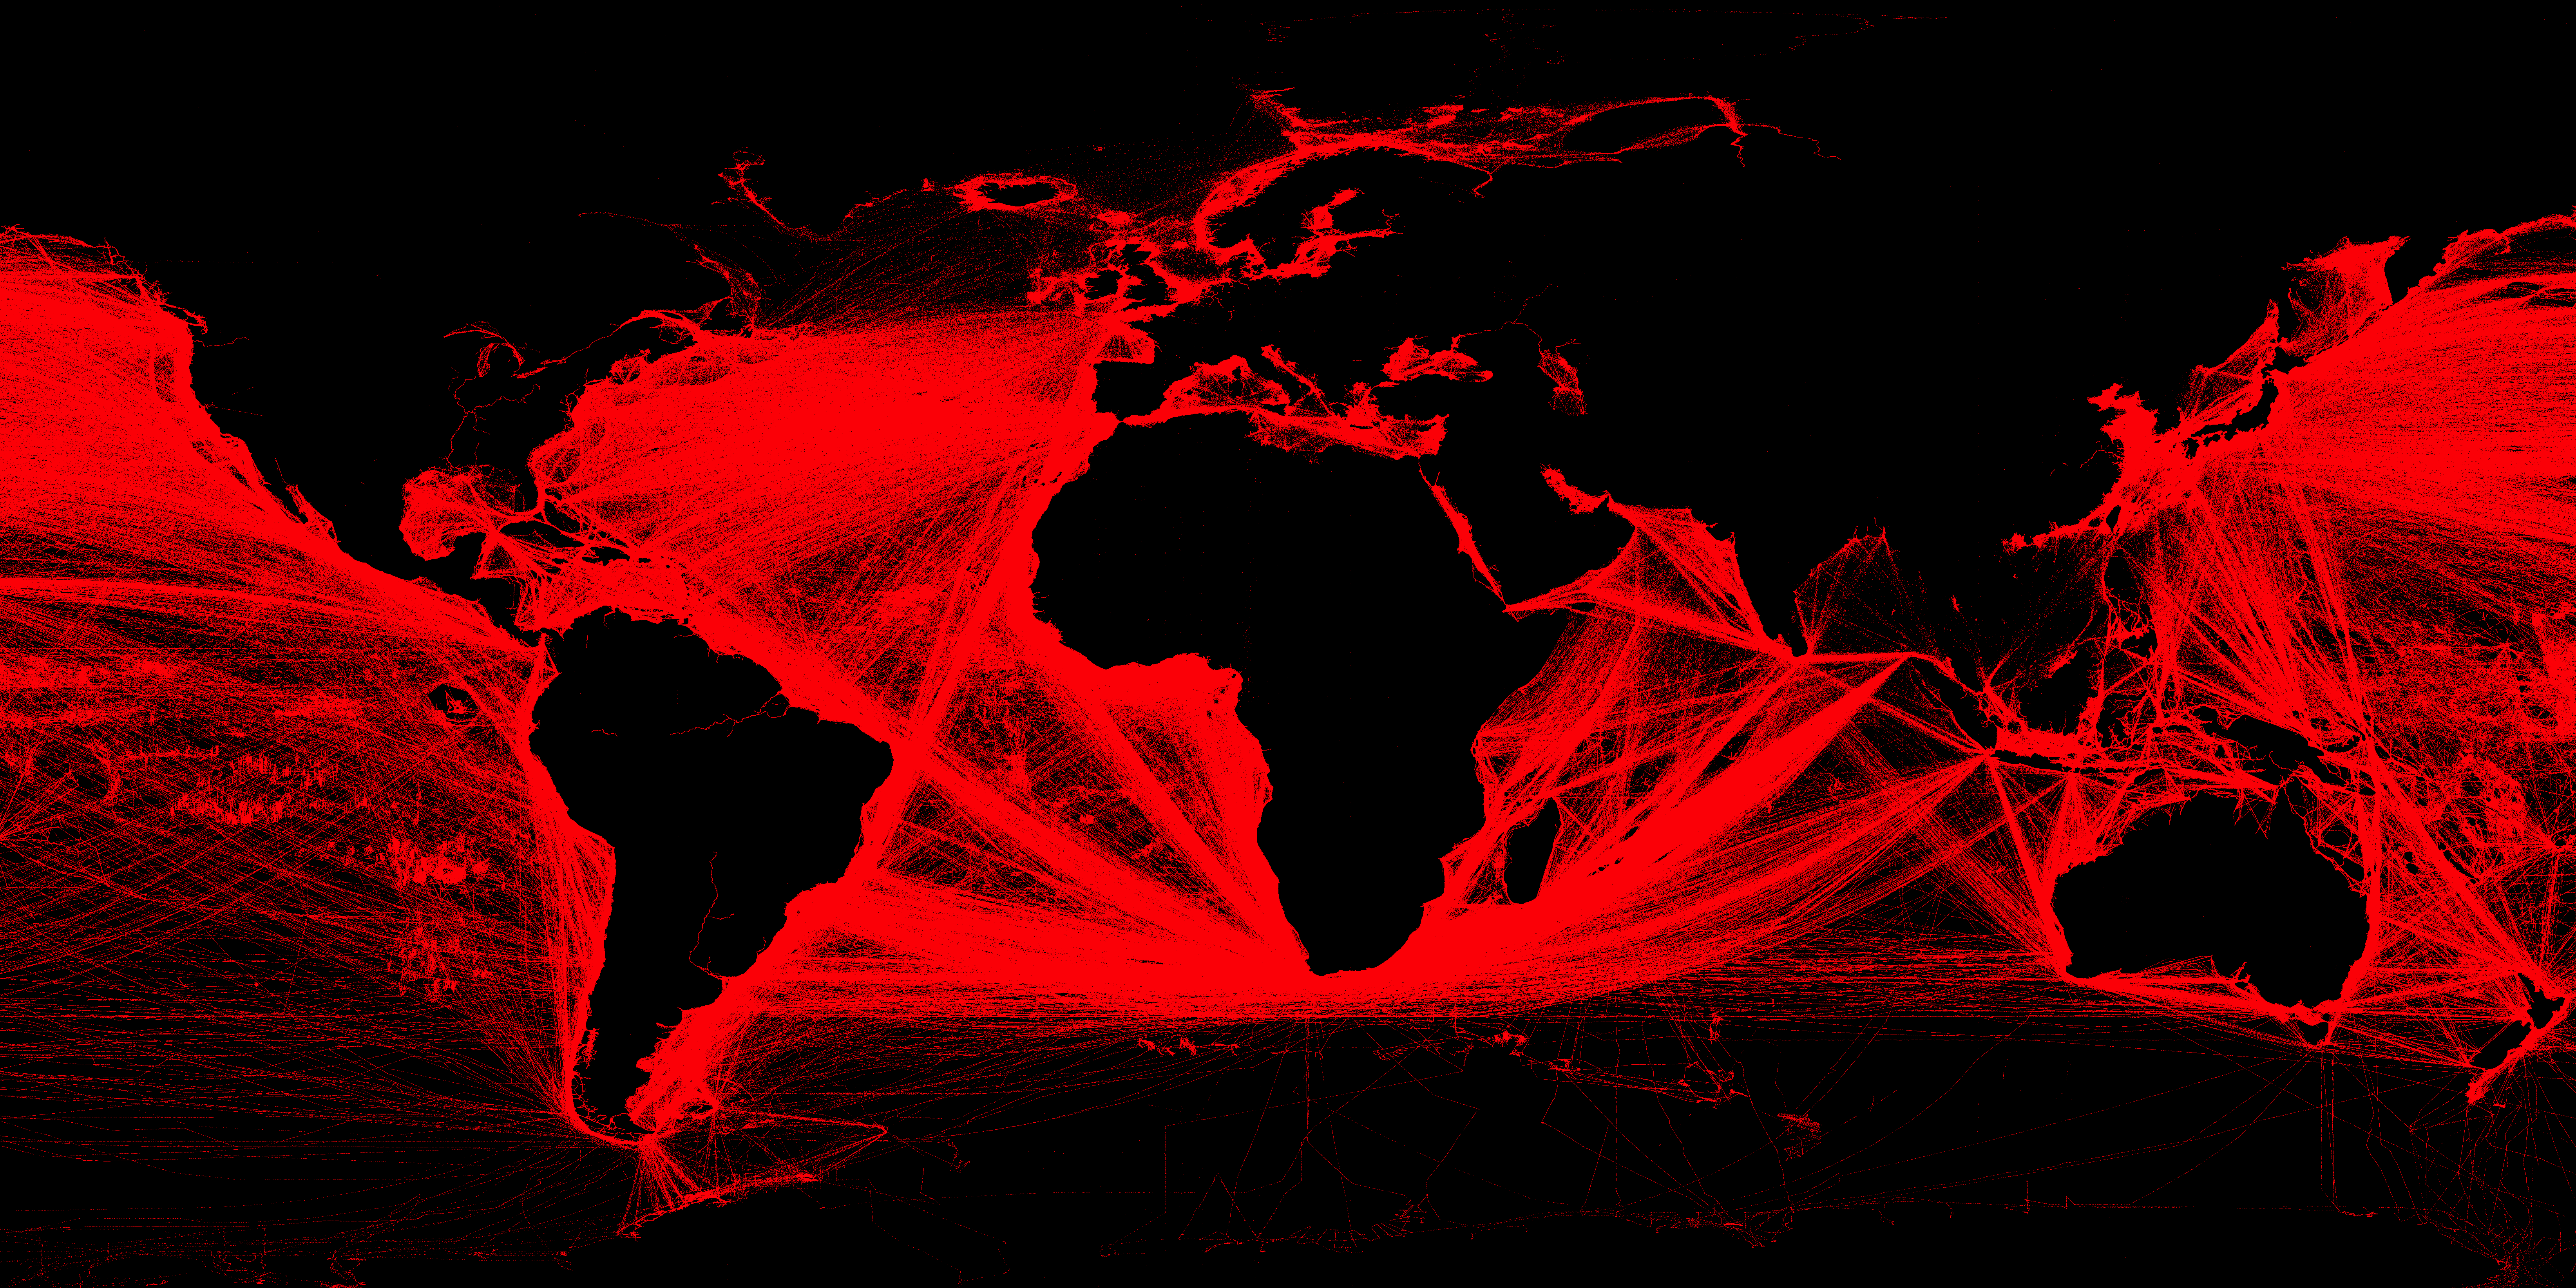
\includegraphics[width=1.0\textwidth]{figures/ais.png}
    \caption{Vessel positions derived from 200 million AIS positional reports}
    \label{fig:ais_positions}
\end{figure}

As already mentioned in \cref{sec:topics_covered}, \acrfull{ais} was initiated by \acrfull{imo} and since 2004 every commercial and passenger vessel exceeding 299 \acrfull{gt} is required to carry an \acrshort{ais} transmitter. These transmitters broadcasts \acrshort{ais} messages following the \gls{aivdm} protocol. The \gls{aivdm} protocol contains two main types of reports: positional and static. The positional reports contains automatically collected information such as the transmitting vessel's \acrfull{mmsi} number, the current timestamp, and the vessel's current navigational data including the current geographical coordinates, \acrfull{sog}, \acrfull{cog}, true heading, \acrfull{rot}, and more. The static reports contain additional information about the vessel and its current voyages, some of which are input manually such as the vessel's \acrshort{imo} number, name, dimensions, draft, intended destination, and \acrfull{eta}.

As an example, \cref{fig:ais_positions} shows a visualization of 200 million \acrshort{ais} randomly chosen positional reports from a collection of historical \acrshort{ais} positions for global collection of shipping vessels. In relation, the historical \acrshort{ais} dataset used in this thesis consists of more than one billion records ranging from December 2019 to March 2021.

Regarding vessel identification in the \gls{aivdm} protocol, there are mainly two values that are unique to a given vessel: the \acrshort{mmsi} and \acrshort{imo} numbers. Either of these should be unique on their own for a given vessel, however, \acrshort{mmsi} numbers can be recycled under certain conditions such as when a vessel is put out of commission while the \acrshort{imo} number is specific to a vessel's hull. Therefore, \acrshort{imo} is the preferred identifier, however, since the \gls{aivdm} protocol divides these identifiers into positional and static reports, both need to be considered in order to use both static and positional \acrshort{ais} information.

Since \acrshort{mmsi} values can be recycled, a mapping between \acrshort{mmsi} and \acrshort{imo} is required. Throughout this thesis, this mapping is provided by \acrfull{mo} and based on the latest combination of \acrshort{imo} and \acrshort{mmsi} values found in the \acrshort{ais} data. This mapping is somewhat flawed as there could be different combinations between the same \acrshort{imo} and different \acrshort{mmsi} values throughout the historical dataset. However, recycled \acrshort{mmsi} is a rare occurrence in the \textit{1.5} years of historical data provided, thus, the mapping is considered sufficient for the purpose of the thesis but could yield potential issues for a few number of vessels.

\section{Initial data foundation}
\label{sec:initial_data_foundation}

This section describes the form and meaning of the data that forms the foundation of the thesis' proposed solution. The data is provided by the collaborative company \acrfull{mo} to the author.

\subsection{Vessel departure and arrival detection}
\label{sec:vessel_transitions}

\acrshort{mo} collects live \acrshort{ais} messages provided by different sources, and in addition, they keep track of their navigational statuses as they are transmitted in the \gls{aivdm} protocol. These status attributes describe the current navigational state of the vessel for purposes of planning and security. Implicitly, these messages can indicate that a vessel has arrived or departed from a given port which can be used to detect voyages. When a vessel has concluded its journey and arrives at a port, the navigational status is changed to \textit{"MOORED"}, and when departing a port, the status is changed to \textit{"UNDERWAY USING ENGINE"} or \textit{"UNDERWAY SAILING"}. There are also other navigational statuses that could be relevant for voyage information such as \textit{"AT ANCHOR"} which could indicate that a vessel is bunkering (refueling) or is waiting for access to a berth that is congested.

\begin{table}
    \centering
    \small{\begin{tabular}{l l}
    \toprule
        \textbf{Status} & \textbf{Description} \\ \midrule
        0 & Under way using engine \\ \midrule
        1 & At anchor \\ \midrule
        2 & Not under command \\ \midrule
        3 & Restricted manoeuverability \\ \midrule
        4 & Constrained by her draught \\ \midrule
        5 & Moored \\ \midrule
        6 & Aground \\ \midrule
        7 & Engaged in Fishing \\ \midrule
        8 & Under way sailing \\ \midrule
        9--13 & Reserved for future use \\ \midrule
        14 & AIS-SART is active \\ \midrule
        15 & Not defined (default) \\ \bottomrule
    \end{tabular}}
    \caption{Available navigational statuses in the \gls{aivdm} protocol.}\label{tab:nav_stats}
\end{table}

\cref{tab:nav_stats} shows all the available statuses that vessels can emit in the \gls{aivdm} protocol. Currently, transitions from a status that indicates that a vessel is moving to the status \textit{"MOORED"}, and from \textit{"MOORED"} to moving are collected and labeled as arrivals and departures from or to the closest port within a given radius. This has proven to be a sufficient method of identifying voyages although it is dependent on the quality of the manually managed status value. Using this approach, voyages are defined by subsequent departure and arrival events, and positions between such events are collected as the voyage's trajectory. As this definition is based on transitioning navigational statuses, throughout this thesis, the concept is referred to as \glspl{transition}.

\subsection{Additional vessel information and segmentation}
\label{sec:vessel_info_segments}

\acrshort{mo} has implemented a system for categorizing vessels into different segments, subsegments, and further variations. These segmentations are based on various factors such as the dimensional data provided by \acrshort{ais} messages as well as technical vessel description provided by external sources and manual user input. One factor for defining vessels' segments can be found in the vessel type from the \gls{aivdm} protocol. However, the most important factor is input from external sources such as IHS Merkit\footnote{\url{https://ihsmarkit.com/index.html}} and DNV\footnote{\url{https://www.dnv.com/}}. This provides a better segmentation than the values provided in the \gls{aivdm} protocol which only provides a much broader definition such as whether the vessel carries passengers, dry cargo, or is a tanker vessel.

For sub-segments, the most important inputs are cargo capacity and carry range, measured in \acrshort{dwt}. This segmentation of vessels is highly relevant to voyage patterns as vessels of different types and sizes travel to different ports and countries for different shipping companies. This is further shown in \cref{fig:segment_map} which shows, from an image of \acrshort{mo}'s web platform, how different sub-segments of the dry bulk cargo segment travels in different areas of the world. Since this categorization provides valuable insights into voyage patterns, vessel segmentation values are included in this thesis's proposed approach to vessel destination prediction.

\begin{figure}[htbp]
    \centering
    \includegraphics[width=1.0\textwidth]{figures/segment_map}
    \caption{\acrfull{mo}’s segmentation of vessels where yellow vessels are smaller than reds}
    \label{fig:segment_map}
\end{figure}

In addition to segment information, \acrshort{mo} has done extensive work into gathering vessel information for their global collection of vessels via sources such as IHS Merkit and DNV. This information is publicized in their software solution where users can suggest changes to this public information which are validated by \acrshort{mo} and applied if the information is valid. The extensive information collected for individual vessels creates a big potential for data analysis and developing \acrshort{ml} models that are highly aware of specific vessels and how they travel. However, in this thesis, the main focus is on vessel segmentation when developing the proposed solution. This data is later referred to as vessel segments and includes both the vessels' segment and sub-segment.

\subsection{Shipping ports}
\label{sec:shipping_ports}

\acrshort{mo} has an extensive port database containing more than 5600 ports. From sources such as UNECE, it is possible to find a vast number of ports, however, only a subset of the world's known ports are used by \acrshort{mo} as these are considered relevant shipping ports. A port is deemed relevant if it offers loading, unloading, or bunkering services and has seemingly valid coordinates and identifiers. The process of determining what ports are relevant shipping ports is a continuous manual process in \acrshort{mo} and it ensures that the available selection of ports is highly relevant for the industry.

Furthermore, all ports are identified by their \gls{locode}. This is a five-letter unique identifier provided and managed by the United Nations (UN). In the five-letter code, the first two indicate the port's country of origin, while the three last indicate a more specific location within the origin country. As an example, the \gls{locode} for the port of Oslo is \texttt{NOOSL} where ``NO'' stands for Norway, and ``OSL'' stands for Oslo. For comparison, a similar system is used for international airports. For this thesis, only the 5600 relevant ports that are considered relevant by \acrshort{mo}'s standards are used in the analysis.

\section{Application challenges}

Throughout the development process of the proposed solution, various implementation, or application challenges arose and were handled. This section aims to describe the background of these issues to help the reader understand the challenges and their respective solutions.

\subsection{AIS data quality}

One important issue to address is the quality of the underlying dataset. The \acrshort{ais} standard is globally adopted and enforced for commercial vessels, however, it lacks standardization for manually managed attributes. This issue affects the chosen voyage definition as it relies on the navigational status in the \acrshort{ais} data. For instance, if vessels neglect to change their signals, their defined voyage trajectories will not properly reflect a commercial voyage and might produce trajectories that are hard to compare with other historical trajectories. Based on manual inspection, vessels seem to be more consistent at changing their statuses from \textit{underway using engine} to \textit{moored} when arriving at a port, than the opposite when departing. This can lead to voyages beginning at some distance away from the departure port while ending more accurately at the arrival port.

\acrshort{ais} data transmitted is collected by either land-based base stations or orbiting satellites depending on the positions of the vessels. The geographical data transmitted is mostly reliable, however, as satellites have different orbits, there are gaps in their coverages. Vessels might travel up to several hours before a satellite collects their transmitted \acrshort{ais} data. There can also be issues with data transmitted in congested areas due to interference from other vessels. Some of these issues cannot be avoided yet affects the outcome of the work conducted in this thesis, however, some issues are identifiable in the historical data and can be managed for analytical purposes. For example, one issue with fluctuations in trajectories was identified and solved in this thesis as described in \cref{sec:traj_validation}.

\subsection{Categorical label encoding}
\label{sec:label_encoding}

Categorical values are values that are a subset of a finite number of possible values, while numerical values have infinite possible values. The thesis problem can be formulated as a multi-class classification problem since the predicted arrival port is a single value in a finite set of ports. \acrshort{ml} models often perform better on, or expect, numerical values in their training datasets\footnote{\url{https://www.mygreatlearning.com/blog/label-encoding-in-python/}}. Therefore, it is common practice to use a form of encoding of the categorical values to transform them into numeric values. There are several different methods of achieving this, however, two common methods are ``Label Encoding'', and ``One-Hot Encoding''. In label encoding, each value in a category is transformed into a numerical value ranging from 0 to the number of unique values in the column. This is a simple and practical encoding method, however, since the categorical values are now numeric, implicitly, the \acrshort{ml} might misunderstand the data to be ordered and derive meaning from the numerical relationships. In one-hot encoding, when a column of data is encoded, the column is split into multiple columns for each different category in the column. Then, the values are replaced by ones and zeros indicating what column contains that value. This solves the issue with implicit patterns in numerical values. However, with high cardinality datasets, \acrshort{ml} models struggle with the sparsity and the large number of features that are generated, and can even perform worse than label encoding in some instances\footnote{\url{https://towardsdatascience.com/d64b282b5769}}.


\subsection{Imbalanced datasets and sampling methods}

Imbalanced datasets are usually problematic in \acrshort{ml} as models see more of certain samples than others making the model biased toward the more frequent outcomes. This can also lead to misleading accuracy values as, during the evaluation process, some values occur more often than others. For example, consider a binary classification problem where the arrival port is either port A or port B. If the dataset contains 90 samples where the arrival port was port A and 10 where it was port B, a simple function could be implemented that always predicts the arrival port to be port A without considering the input values and the ``model'' would have an apparent accuracy of \textit{90\%}. However, this accuracy would be misleading as the model will never predict port B as the arrival port. The same phenomena can occur in \acrshort{ml} models that are trained on imbalanced datasets. Some \acrshort{ml} models deal with the problem of imbalance better than others, especially decision tree ensemble methods such as the Random Forest (RF) model, however, these models might still struggle with highly imbalanced datasets.

There are several methods of dealing with imbalanced datasets including providing models with predefined weights, however, not all models provide this option. For a more general approach, it is possible to manipulate the dataset before training in an attempt to balance the classes. This can be achieved through sampling the dataset in a manner that produces a more balanced frequency of the outcome values. The two methods in question are minority oversampling and majority undersampling. Minority oversampling is a procedure where the minority classes, or target values, are duplicated while majority undersampling consists of removing majority classes until the dataset contains an equal number of classes. On a general basis, these methods have their accompanying caveats. For instance, when oversampling the minority classes, the model has a greater chance of overfitting as it sees a high number of the same samples. In contrast, when undersampling majority classes important relationships in the datasets might be removed along with the samples of the majority classes.

There have been some attempts at minority oversampling without simply duplicating information. A popular approach called \acrfull{smote} \parencite{Chawla2002} achieves this by synthetically generating new samples based on closely related samples in the dataset. For majority undersampling, Edit Nearest Neighbor (ENN) evaluates \textit{k} nearest neighbors to find misclassified samples and removes them. This enables majority undersampling with less risk of removing important relationships in the dataset. \cite{cv_imbalance} describes possible implications that oversampling may have on imbalanced dataset evaluation. They found that datasets oversampled using \acrshort{smote} can lead to some misleading evaluation results such as that of an over-optimistic evaluation process. When any oversampling technique has been applied to a dataset, there is a risk of the evaluation sets containing many similar or duplicate values as the training set, thus, the model is evaluated using samples it has already seen during the training process. In general, they found that using a combination of over and undersampling using \acrshort{smote} and Tomek Links \parencite{tomek} respectively produced the most reliable results.

\subsection{Model evaluation}
\label{sec:model_evaluation}

After a \acrfull{ml} model has been trained it must be validated properly in order to determine its real performance. The simplest evaluation process consists of dividing the full dataset into a training and a test dataset by a certain sample ratio, commonly \textit{80\%} train and \textit{20\%} test data. This is important as to not evaluate the model using samples it has already observed in the training process and to ensure that the model performs as expected on previously unseen samples. When the trained model performs well on the training data, but not on previously unseen samples, the model is overfitted. In such cases, the model essentially remembers the entire training dataset but has not learned it, so it cannot be applied to previously unseen samples. Moreover, to ensure that the selected portion of test data was representative of the dataset, \textit{k-Fold cross-validation} can be employed \parencite{ghojogh2019theory}. In this process, the full dataset is divided into \textit{k} parts of equal size, and the model is trained \textit{k} times, using one different part as test data and the remaining as training data for each training process. The average accuracy value can then be extracted from each of the training rounds to determine a more balanced accuracy value. Furthermore, if the level of accuracy differs significantly per training round, or the standard deviation of accuracy is large, it indicates that the model can be overfitting in the training process.
